\section{Astrophysical Models}
\label{sec:models}

%==============================================================================
\subsection{Basic Assumptions}
\label{sec:basic}

In this paper, we assume the mass of and distance to \sgra are
\begin{align}
  \mbh &= 4.14  \times 10^6 \msun, \label{eq:mass} \\
  D    &= 8.127 \kpc,              \label{eq:dist}
\end{align}
which are approximately the mean of the values reported by \citet{2019Sci...365..664D} and \citet{2019A&A...625L..10G}, which differ by about 4\%.  The distance is consistent with maser parallax measurements \citep{2019ApJ...885..131R}.

In this paper we assume that \sgra is a black hole described by the Kerr metric.
The black hole dimensionless spin, $\abh \equiv Jc/G\mbh^2$, is a free parameter with $-1 < \abh < 1$;  $J$, $G$, and $c$ are the black hole spin angular momentum, gravitational constant, and speed of light, respectively.
Following \citet{M87PaperV}, hereafter \citetalias{M87PaperV}, we use
$\abh > 0$ to indicate that the angular momentum of the accretion flow and black hole are parallel (the accretion flow is ``prograde'') and
$\abh < 0$ to indicate that the angular momentum of the accretion flow and black hole are antiparallel (``retrograde'').\footnote{For tilted disks the sign of $\abh$ is the sign of ${\bf J}\cdot{\bf L}$ where ${\bf J}$ is black hole spin angular momentum and ${\bf L}$ is accretion flow orbital angular momentum.}

Using the above mass and distance, the implied
characteristic length:
\begin{equation}
r_\mathrm{g}         \equiv G\mbh/ c^2    \simeq 6.1\times10^{11}\cm,
\end{equation}
characteristic time:
\begin{equation}
t_\mathrm{g}         \equiv G\mbh/ c^3    \simeq 20.4\sec,
\end{equation}
and
angular scale:
\begin{equation}
\vartheta_\mathrm{g} \equiv G\mbh/(c^2 D) \simeq 5.03\uas.
\end{equation}
The expected diameter of the black hole shadow is $2\sqrt{27} G\mbh/(c^2 D)$ for $\abh = 0$.  For $|\abh| > 0$ the shadow is noncircular and its size and shape depend on $\abh$ and inclination $i$ (the angle between the line of sight and the spin axis); its width can be as small as $9 G\mbh/(c^2 D)$ for $\abh = 1$ and $i = 90\deg$ \citep{1973blho.conf..215B}.

If the emitting plasma is ionized hydrogen (electron-proton plasma) then the Eddington luminosity is:
\begin{equation}
L_\mathrm{Edd} \equiv 4\pi G\mbh c m_p/\sigma_\mathrm{T} = 5.2 \times 10^{44}\erg \sec^{-1},
\end{equation}
where symbols have their usual meaning.
The corresponding Eddington accretion rate is
\begin{equation}
\dot\mbh_\mathrm{Edd} \equiv L_\mathrm{Edd}/(0.1 c^2) = 5.8 \times 10^{24} \gm \sec^{-1} = 0.09 \msun \yr^{-1},
\end{equation}
where the nominal efficiency is 10\% and the Eddington ratio:
$L_\mathrm{bol}/L_\mathrm{Edd} = 1.9 \times 10^{-10} (L_\mathrm{bol} \ergps /10^{35} \ergps)$.
In a quiescent, non-flaring state, the bolometric luminosity of \sgra is $L_\mathrm{bol} \sim 10^{35}\ergps$, resulting in an extremely small Eddington ratio.
In what follows we assume that radiative cooling of plasma around the black hole can be neglected (which is partially justified later) and that the emergent radiation can be calculated in post-processing.

%==============================================================================
\subsection{One-Zone Model Estimates}

Here we use a simple, one-zone model to motivate the more complicated models that follow, as in \citetalias{M87PaperV}.  These results follow one-zone models developed in the literature over many decades \citep[e.g.][]{1996IAUS..169..169F}.

Consider a spherical, uniform plasma of radius $r = 5\rg$, comparable to the observed size of \sgra at $230\GHz$ (\citetalias{PaperIII}, \citetalias{PaperIV}), with uniform magnetic field oriented at $\pi/3$ to the line-of-sight.  In turbulent astrophysical plasmas it is common for  the gas pressure to be comparable to the magnetic pressure, and we assume that here: $n_i k T_i + n_e k T_e = B^2/(8\pi)$, where $T_i \equiv$ ion temperature, $T_e \equiv$ electron temperature, $B \equiv$ magnetic field strength in Gauss.  The plasma is collisionless (checked below), and it is plausible that the ions are preferentially heated, so we assume $T_i \sim 3 T_e$.  If the ions are sub-virial by a factor of about $3$, commonly seen in relativistic MHD simulations, then $(3/2) k T_i \sim (1/3) (1/2) (G M m_p/r)$.  Then the ions are nonrelativistic and the electrons are relativistic, with $\Theta_e \equiv  k T_e / m_e c^2 \sim 10$.

Using a thermal synchrotron emissivity $j_\nu$ \citep[e.g.,][]{2011ApJ...737...21L} and assuming optically thin emission, the flux density from a uniform sphere, $F_\nu = (4/3)\pi r^3 j_\nu D^{-2} 10^{23}\,\mathrm{Jy}$.  Setting $F_\nu = 2.4\,\mathrm{Jy}$ (the average measured by ALMA during the 2017 campaign; \citealt{Wielgus2022}) yields a nonlinear equation for the electron density, $n_e$, with solution
\begin{align}
  n_e &\simeq 1.1\times10^6\cm^{-3},\\
  B   &\simeq 30\,\mathrm{Gauss}.
  \label{eq:onezone}
\end{align}
The synchrotron optical depth $\tau_\mathrm{sync} = r j_\nu/B_\nu \simeq 0.4$, where $B_\nu$ is the Planck function, so the optically thin approximation is marginal.
These values are consistent with $n_e$ and $B$ of a similar one-zone model fitted to archival \sgra millimeter spectrum \citep{2019ApJ...881L...2B}.
%MM: fit of similar one zone model to Terahertz spectrum from ALMA infers ne=2-5x10^6 cm^-3, B=10-50 Gauss, T_e=1-3x10^11 K => Thetae=16-50
% CFG: I've placed a mathematica script implementing the one zone model in eht.astro.illinois.edu://bd4/eht/paperV/OneZoneThin.ma

The one-zone model has electron scattering optical depth  $\tau_e \sim \sigma_T n_e r \simeq 2\times10^{-5}$ and thus a small Compton parameter: $y = 16 \Theta_e^2 \max(\tau_e,\tau_e^2) \simeq 0.03$.  Synchrotron cooling therefore dominates Compton cooling.

The synchrotron cooling timescale $t_\mathrm{cool} \equiv u/\Lambda$ where $u_e = 3 n_e k T_e$ is the electron internal energy and $\Lambda \simeq 5.4 B^2 e^4 n_e \Theta_e^2 /(c^3 m_e^2)$ is the synchrotron cooling rate for a thermal population of electrons with $\Theta_e \gtrsim 1$ (see Appendix~A in \citealt{2011ApJ...735....9M}; finite optical depth reduces $\Lambda$).
The cooling time is therefore $t_\mathrm{cool}=2.3 \times 10^4\sec \simeq 1.1 \times 10^3 \tg$ which is longer than the inflow timescale $r/v^r \sim r^{3/2}$.  This suggests that radiative cooling can be neglected in the plasma models \citep[more detailed calculations confirm this estimate][]{2012MNRAS.426.1928D,2020MNRAS.499.3178Y}.\footnote{Notice that if \sgra is fed by stellar winds then the inflowing plasma may be mainly helium \citep{2019MNRAS.482L.123R}; this changes the one-zone model slightly. Helium accretion is discussed in detail in \citep{Wong_2022}.}

The one-zone model $n_e, \Theta_e$ imply that the mean free path to Coulomb scattering is large compared to $\rg$, i.e. the source plasma is collisionless.
At $\Theta_e \sim 1$, for example, the Coulomb scattering cross section is comparable to the Thomson cross section, and therefore the mean free path $\sim \tau_e^{-1} \rg$.
The electron-ion Coulomb scattering timescale is also long, and the electrons and ions are therefore poorly coupled.
This is consistent with our assumption of a two-temperature  plasma where electrons are cooler than the ions \citep{1976ApJ...204..187S,1977ApJ...214..840I, 1982Natur.295...17R} and motivates consideration of
nonthermal (unrelaxed) electron distribution functions \citep[see][]{2000ApJ...541..234O, 2009ApJ...701..521C, 2014A&A...570A...7M, 2018A&A...612A..34D, 2021arXiv211102518F, 2021NatAs.tmp..218C, Chatterjee2021, 2021arXiv211203933E, Scepi2021}.

%==============================================================================
\subsection{Numerical Models of the Inner Accretion Flow}

% CFG new version
% do we need the rmax column?  perhaps provide torus information?
\begin{deluxetable*}{cccccccccc}
  \label{tab:GRMHDmodels}
  \tablecaption{EHT GRMHD Simulation Library}
  \tablehead{
    \colhead{Setup}                &
    \colhead{Code}                 &
    \colhead{$\abh$}               &
    \colhead{Mode}                 &
    \colhead{$\Gamma_\mathrm{ad}$} &
    \colhead{$t_\mathrm{final}$ }  &
    \colhead{$r_{\rm in}$}         &
    \colhead{$r_{\rm max}$}        &
    \colhead{$r_{\rm out}$}        &
    \colhead{Resolution}%
  }
  \startdata
  torus    & {\kharma}$^a$ & 0, $\pm 0.5$, $\pm 0.94$   & MAD/SANE & $\frac{4}{3}/\frac{4}{3}$  & 30,000  & --- & --- & 1000     & $288\times128\times128$     \\
  torus    & \bhac$^b$     & 0, $\pm 0.5$, $\pm 0.94$   & MAD/SANE & $\frac{4}{3}/\frac{4}{3}$  & 30,000  & --- & --- & 3333     & $512\times192\times192$     \\
  torus    & \hamr$^c$     & 0, $\pm 0.5$, $\pm 0.94$   & MAD/SANE & $\frac{13}{9}/\frac{5}{3}$ & 35,000  & --- & --- & 1000/200 & $348/240\times192\times192$ \\
  torus    & \koral$^d$    & \!\!\!\!\!\!0, $\pm 0.3$,  %
$\pm 0.5$, $\pm 0.7$, $\pm 0.9$\!\!\!\!\!\!\!\!\!\!\!\! & MAD      & $\frac{13}{9}$             & 101,000 & --- & --- & 100,000  & $288\times192\times144$     \\
  tilted   & \hamr$^e$     & $0.94$                     & IN-SANE  & $\frac{5}{3}$              & 105,000 & --- & --- & 100,000  & $448\times144\times240$     \\
  wind-fed & \athenapp$^f$ & 0                          & ILAF     & $\frac{5}{3}$              & 20,000  & --- & --- & 2,400    & $356\times128\times128$
  \enddata
  \tablecomments{Summary of the EHT \sgra GRMHD simulation library.
    The last column is $N_1 \times N_2 \times N_3$, with coordinate
    $x_1$ monotonic in radius, $x_2$ monotonic in colatitude $\theta$,
    and $x_3$ proportional to longitude $\phi$.
    The first four entries use aligned torus initial conditions.
    The last two entries are tilted accretion models and two
    realizations of the Wind-fed accretion model which differ in
    stellar wind magnetization.
    Times are given in units of $G M/c^3 = 20.4\sec$ and radii in units
    of $G M/c^2$.%
  }
  \tablerefs{
    $^a$see \citet{2021JOSS....6.3336P}; \kharma is a GPU-enabled version of the {\tt iharm3d} code.
    $^b$\citet{2017ComAC...4....1P, Olivares2019}.
    $^c$\citet{2021arXiv210812380N}.
    $^e$\citet{2019arXiv191210192L, Chatterjee2020}.
    $^f$\citet{2016ApJS..225...22W, 2020ApJ...896L...6R}.%
  }
\end{deluxetable*}

% version as of 1/23/22
%\begin{deluxetable*}{cccccccc}
%  \tabletypesize{\footnotesize}
 % \renewcommand{\arraystretch}{1.1}
  %
%  \tablehead{
%    \colhead{Setup/Code}                  &
%    \colhead{BH spin $\abh$}                     &
%    \colhead{Mode}                       &
%    \colhead{$\Gamma_\mathrm{ad}$}       &
%    \colhead{\!\!\!\!\!\!$t_\mathrm{final}$ [$\rg$]} &
%    \colhead{$r_{\rm max}$ [$\rg$]\!\!\!\!\!\!}         %      &
%    \colhead{Resolution}                 &
%    \colhead{Reference}
%  }
%  \startdata
%  \begin{tabular}{@{}c@{}} torus / \\ \kharma \end{tabular} & 0,$\pm1/2$,$\pm15/16$                 & MAD/SANE     & $\frac{4}{3}/\frac{4}{3}$      & 30,000  & 1000     & [288x128x128]     & \!\!\!\!\!\!\!\!\!
%  \begin{tabular}{@{}c@{}c@{}c@{}} This work\\\citet{kharma_2022}\\\citet{Wong_2022} \\ \citet{Dhruv_2022}\end{tabular}\\
% \citet{Wong_2022, Dhruv_2022} \\
%  \begin{tabular}{@{}c@{}} torus / \\ \bhac \end{tabular}   & 0,$\pm1/2$,$\pm15/16$                 & MAD/SANE     & $\frac{4}{3}/\frac{4}{3}$      & 30,000  & 3333     & [512x192x192]     &  \!\!\!\!\!\!\!\!\!
%  \begin{tabular}{@{}c@{}c@{}c@{}} This work \\ \citet{Mizuno2021}\\  \citet{2021NatAs.tmp..218C}\\ \citet{2021arXiv211102518F} \end{tabular}\\
%  \begin{tabular}{@{}c@{}} torus / \\ \hamr \end{tabular}   & 0,$\pm1/2$,$\pm15/16$                 & MAD/SANE     & $\frac{13}{9}/\frac{5}{3}$ & 35,000  & 1000/200 & [348/240×192×192] & This work \\
%  \begin{tabular}{@{}c@{}} torus / \\ \koral \end{tabular}  & \!\!\!\!\!\!\!\!\!
%  \begin{tabular}{@{}c@{}c@{}}   0,$\pm0.3$,$\pm0.5$\\$\pm0.7$,$\pm0.9$ \end{tabular}
%  \!\!\!\!\!\!\!\!\! & MAD          & $\frac{13}{9}$     & 101,000 & 100,000  & [288x192x144]     & \citet{2021arXiv210812380N} \\
%  \begin{tabular}{@{}c@{}} tilted / \\ \hamr \end{tabular}     & $15/16$     & IN-SANE$\times3$      & $\frac{5}{3}$        & 105,000 & 100,000  & [448x144x240]     & \begin{tabular}{@{}c@{}} \citet{Liska2018} \\ \citet{Chatterjee2020}\end{tabular} \\
%  \begin{tabular}{@{}c@{}} wind-fed / \\ \athenapp \end{tabular} & 0           & MAD$\times2$ & $\frac{5}{3}\times2$        & 20,000  & 2,400    & [356x128x128]     & \begin{tabular}{@{}c@{}} \cite{2016ApJS..225...22W} \\ \citet{2020ApJ...896L...6R} \end{tabular}
%  \enddata
  %
  %\tablenotetext{$*$}{Non-standard model.}
%  \caption{Summary of GRMHD simulations in the EHT \sgra GRMHD simulation library.
%    The first four entries are \sgra simulations based on default torus initial conditions.
%   The last two entries are the tilted accretion model and two realizations of the Wind Accretion models which differ in stellar wind magnetization.}
%  \label{tab:GRMHDmodels}
%\end{deluxetable*}

The one-zone model is too simple for comparison with the rich set of observations available for \sgra.  Steady spherical accretion models \citep[e.g.,][]{2019ApJ...885L..33N, 2021arXiv211102178B} go a step beyond the one zone model, incorporating relativistic gravity.  Steady, disk-like (RIAF) accretion models in the Kerr metric go still further and include rotation and departures from spherical symmetry \citep[e.g.,][]{2009ApJ...697...45B, 2009ApJ...706..960H,2018ApJ...863..148P}.
% I think the previous sentence says both analysis spherical and disk can be used for blab blab blab...  Minor edit to retain that meaning.
Steady phenomenological models do not, however, self-consistently capture fluctuations in the flow.  That requires either a statistical model \citep{2021ApJ...906...39L} or a time-dependent numerical simulation.
%\ckc{May be also say they don't self-consistently capture turbulence for transport.}
Here we use numerical simulations, adopt an ideal GRMHD model for the flow, use simple parameterized models to assign an electron distribution function, and solve the radiative transfer equation along geodesics to produce simulated images.

%------------------------------------------------------------------------------
\subsubsection{Plasma Flow Model}

We model the plasma flow around \sgra using ideal, non-radiative GRMHD.  We assume the gravitational field
is described by the Kerr metric, with mass from Equation~(\ref{eq:mass}) and with $\abh$ a free parameter \citep[see e.g.,][]{1999ApJ...522..727K,2003ApJ...589..444G, 2003ApJ...589..458D, 2005ApJ...635..723A, 2007A&A...473...11D}.

We integrate the GRMHD equations in three spatial dimensions using multiple algorithms:
\kharma   \citep{2021JOSS....6.3336P},
\bhac     \citep{2017ComAC...4....1P},
\hamr     \citep{Liska2019},
\koral    \citep{2013MNRAS.429.3533S}, and
\athenapp \citep{2016ApJS..225...22W};
see \citet{2019ApJS..243...26P} and \citet{Olivares_et_al} for comparisons of GRMHD codes.
All simulations assume constant adiabatic index  $\Gamma_\mathrm{ad}$.

The initial conditions for most GRMHD simulations  are a constant-angular-momentum hydrodynamic equilibrium, the Fishbone-Moncrief torus \citep{1976ApJ...207..962F}.  In all except the \hamr-Tilted models the torus orbital angular momentum is either parallel or antiparallel to the black hole spin.  The torus is seeded with a weak, poloidal magnetic field.  There are variations in the radius of the torus pressure maximum (from $\sim 15-40$), in peak temperature, in  adiabatic index, and in field configuration between simulations.  Despite these variations the radiative models based on these simulations are in broad agreement.

The torus initial conditions are motivated by the notion that the near-horizon flow, where most of the emission is generated (\citetalias{M87PaperV}) relaxes to a statistically steady state that is nearly independent of the flow at larger radius.  This notion is challenged in the stellar wind-fed models of \cite{2020ApJ...896L...6R}, which are included in our study.

All simulations are run in variations of Kerr-Schild coordinates, which are regular on the horizon.
Most are run in a variant of spherical polar coordinates.
Unless stated otherwise, boundary conditions are outflow at the inner boundary, located inside the event horizon, outflow at the outer boundary, located at $r_{\rm max} \gtrsim 1000~\rg$, and reflecting boundary conditions at the poles.
Most simulations are evolved to $t_\mathrm{final} = 30,000~\tg$.

Once the evolution has started, a combination of instabilities including the magnetorotational instability \citep[MRI][]{1992ApJ...400..610B} drives the torus to a turbulent, fluctuating state.
If $P_\mathrm{gas} \equiv$ gas pressure and $P_\mathrm{mag} \equiv B^2 / (8\pi) \equiv$ magnetic pressure, the standard accretion flow models can be divided by latitude into three zones:
\emph{i})~an equatorial inflow,
\emph{ii})~a mid-latitude disk wind/corona with  $\beta  \equiv P_\mathrm{gas} / P_\mathrm{mag} \sim 1$, and
\emph{iii})~a polar ``funnel'' with $\sigma \equiv B^2/4\pi \rho c^2 \gg 1$.

The magnetic flux through the horizon divides the outcome into two categories (see, e.g, \citealt{M87PaperV} and \citealt{M87PaperVIII}, hereafter \citepalias{M87PaperVIII}, and references therein): the magnetically arrested disk (MAD) state \citep[e.g.,][]{1974Ap&SS..28...45B, 2003ApJ...592.1042I, 2003PASJ...55L..69N, 2011MNRAS.418L..79T} in which the magnetic flux on the horizon saturates and substantially affects the dynamics of the flow, and the Standard and Normal Evolution (SANE) state \citep[e.g.,][]{2003ApJ...589..444G, 2003ApJ...599.1238D, 2012MNRAS.426.3241N}.
The dimensionless magnetic flux $\phi \equiv \Phi_{\mathrm{BH}} (\dot{M} r_\mathrm{g}^2 c)^{-1/2}$, where $\Phi_{\rm BH}$ is the magnetic flux interior to the black hole equator and $\dot{M}$ is the mass accretion rate through the horizon.
MAD models have $\phi \sim \phi_{\rm crit} \sim 60$.\footnote{In the Lorentz-Heaviside units commonly used in GRMHD simulations $\phi_\mathrm{crit}$ is smaller by a factor of $(4\pi)^{1/2} \simeq 3.545$.}
%\aco{Should we cite the work-in-progress by Narayan about spinup-spindown for MAD models where magnetic flux it can be written as a function of BH spin? I've verified the same tendency for BHAC.}
%\monika{not necessary, this is not established and should be first published we want to limit in prep as much as possible}
In MAD models, magnetic flux accretes onto the hole until $\phi \gtrsim \phi_\mathrm{crit}$, then magnetic flux is expelled from the hole and escapes through the inflowing plasma.  SANE models have $\phi < \phi_\mathrm{crit}$, and most of our standard models have $\phi \sim 1$.

We consider two GRMHD simulations with initial conditions that differ from the fiducial aligned torus: strongly magnetized non-MAD tilted torus simulations \citep{Liska2018, Chatterjee2020} and a model in which \sgra is fed directly by winds from stars in its vicinity \citep{2020ApJ...896L...6R}.
The wind-fed simulations result in a mode of accretion that is similar to MAD but typically has lower mean angular momentum and is less well organized.
The wind-fed models have $\abh = 0$.

The GRMHD simulation library is summarized in Table~\ref{tab:GRMHDmodels}.
In Figure~\ref{fig:GRMHD} we show a few examples of GRMHD simulations for an aligned SANE, an aligned MAD, a tilted torus, and a wind-fed simulation.
The models vary in numerical method and in numerical resolution. We present more information on the numerical methods and models in Appendices~\ref{app:numerical} and \ref{app:variability}.

\begin{figure*}
  \centering
  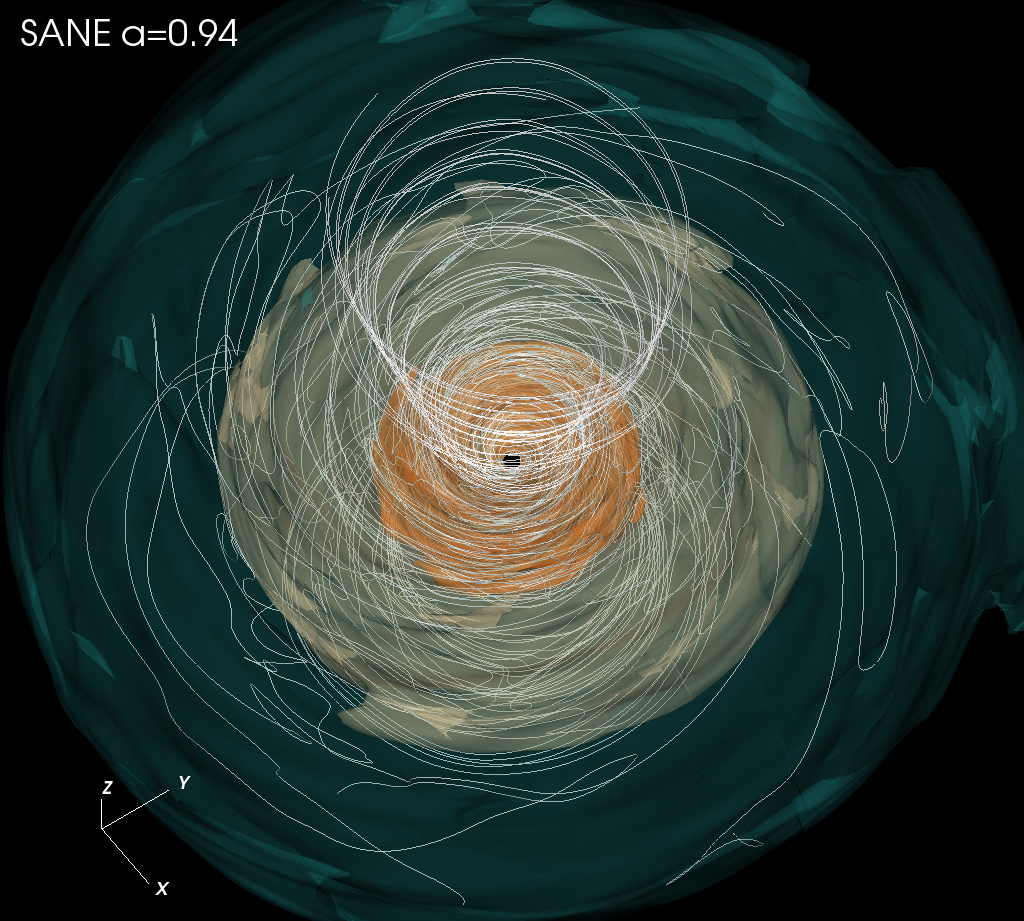
\includegraphics[width=0.425\textwidth]{figures/sane_3D_corrected.png}\hspace{1.5pt}%
  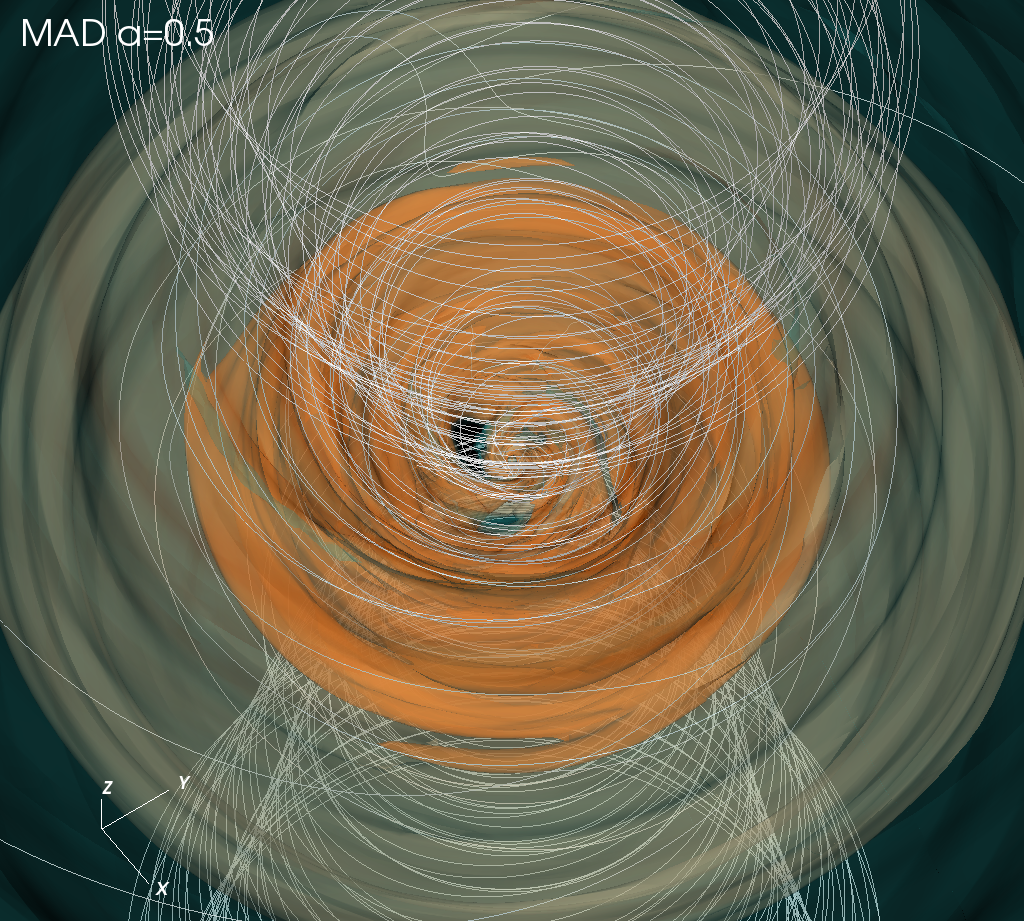
\includegraphics[width=0.425\textwidth]{figures/mad_3D_corrected.png}\\
  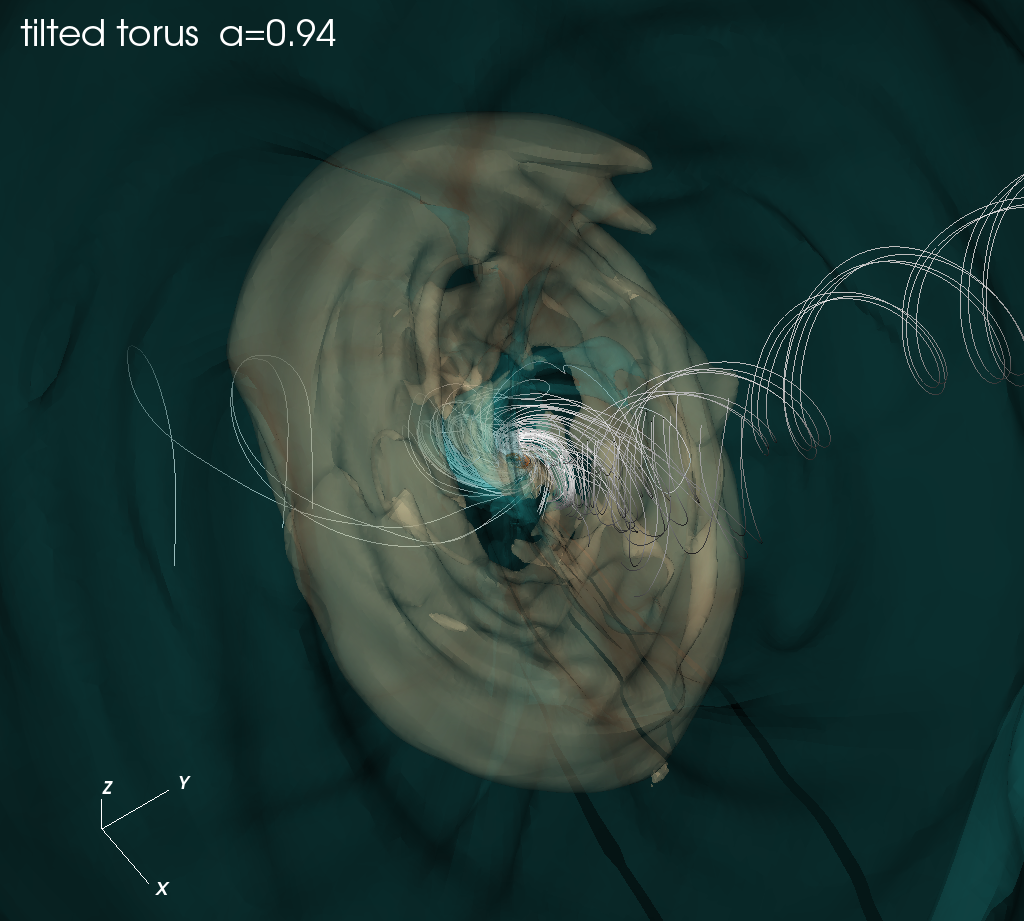
\includegraphics[width=0.425\textwidth]{figures/tilted_3D_corrected.png}\hspace{1.5pt}%
  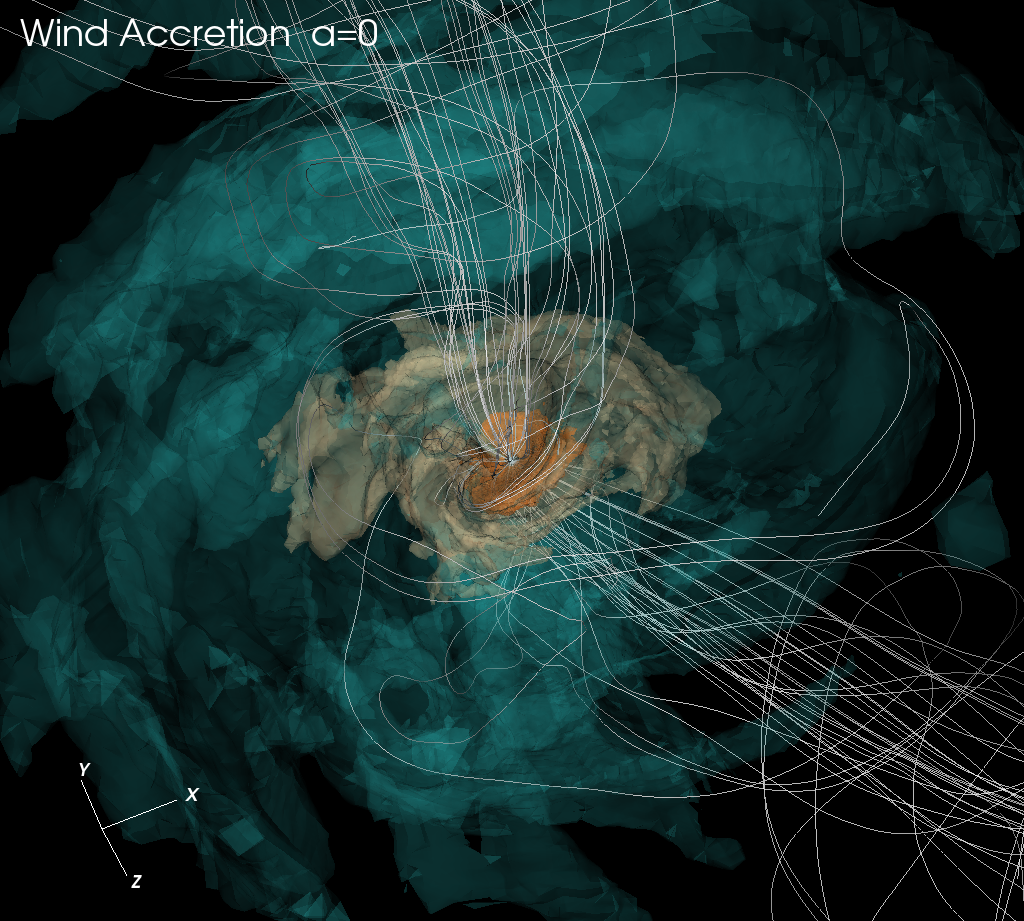
\includegraphics[width=0.425\textwidth]{figures/ressler_3D_corrected.png}
  \caption{3-D overview of selected GRMHD simulations of \sgra in our library.
    The color marks constant dimensionless density surfaces and lines follow magnetic field lines (the magnetic field lines shown are only those which are attached to the inner part of the accretion flow, at $r\approx 5~\rg$).
    Two top panels show accretion simulations with default torus initial condition and
    two bottom panels show non-standard accretion models. In case of spinning black holes, the spin is aligned with z-axis.}
  \label{fig:GRMHD}
\end{figure*}

One critical feature of the GRMHD simulations that is important for the interpretation of our results is the temperature profile.  Figure \ref{fig:grmhd_temp} shows the time- and azimuth- averaged profiles of the midplane dimensionless {\em ion} temperature in a set of aligned GRMHD simulations.  The temperature profiles exhibit strong trends with spin and magnetic state (MAD or SANE) that drives many of the trends seen in the radiative models: MAD models are factor of several hotter than than SANE models and both MAD and SANE become hotter as $\abh$ increases.

\begin{figure*}
  \centering
  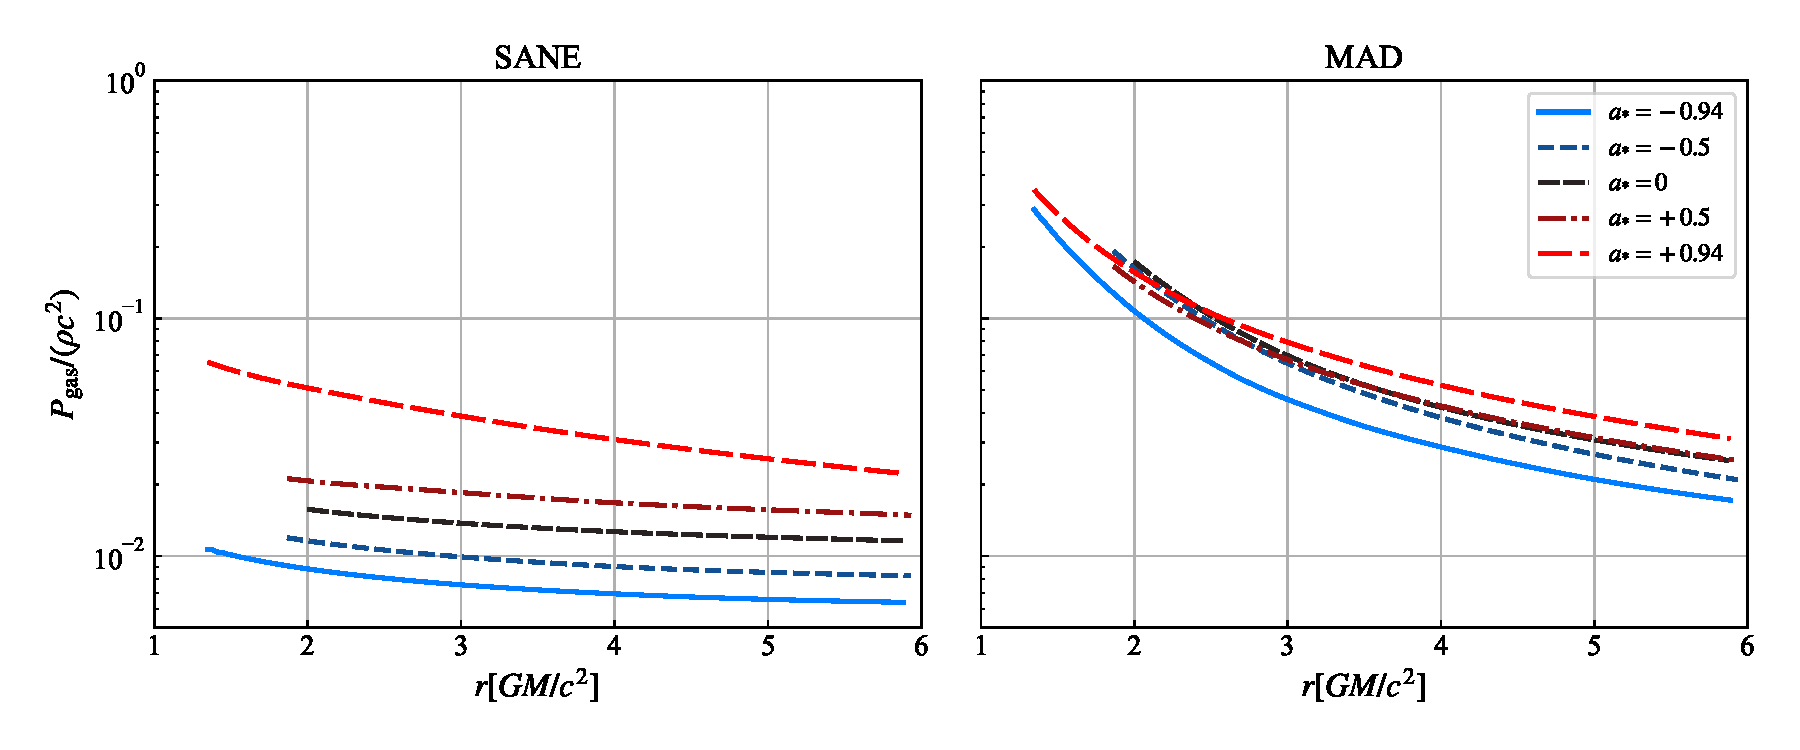
\includegraphics[width=0.9\textwidth]{figures/grmhd_temp.pdf}
  \caption{Time- and azimuth- averaged profiles of midplane dimensionless ion temperature in fiducial GRMHD simulations from \kharma.  Evidently MAD models are hotter than SANE, and both MADs and SANEs grow hotter as the black hole spin $\abh$ increases.  The hottest models are $\abh = 0.94$ MAD models.}
  \label{fig:grmhd_temp}
\end{figure*}

%------------------------------------------------------------------------------
\subsubsection{Radiative Transfer Model}

Synthetic images are generated from the GRMHD simulations in a radiative transfer step.  The transfer step requires:
\emph{i})~a model for the electron temperature and electron distribution function (hereafter eDF);
\emph{ii})~an assignment of a density scale to the GRMHD simulation;
\emph{iii})~a numerical radiative transfer step performed after the GRMHD simulation, assuming that the plasma evolution is unaffected by radiation.

The transfer step requires that we specify any parameters associated with the eDF (e.g. $\Rh$), the inclination $i$ (angle between the black hole spin axis and the line of sight), and an accretion rate or equivalently a density scale, which is not determined by the GRMHD simulation.

%..............................................................................
\subsubsubsection{Electron Distribution Function}
\label{sec:eDF}

In \emph{thermal} models electron energies are distributed into the Maxwell-J{\"u}ttner distribution function:
\begin{align}
  \frac{1}{n_e}\frac{dn_e}{d\gamma} = \frac{\gamma^2 \sqrt{1-1/\gamma^2}} {\Theta_e K_2(1/\Theta_e)} \exp\left(-\frac{\gamma}{\Theta_e}\right);
  \label{eq:thermaleDF}
\end{align}
where $K_2$ is the modified Bessel function of the second kind and $\gamma$ is the Lorentz factor of an electron. Recall $\Theta_e = k_b T_e/(m_e c^2)$, which is determined by the ion-electron temperature ratio $R \equiv T_i/T_e$:
\begin{align}
  T_e=\frac{2 m_p u}{3 k_B \rho (2+R)}.
\end{align}
Here $u$ and $\rho$ are the internal energy density and rest-mass density from the GRMHD simulation, and we assume that the ions are nonrelativistic with adiabatic index is $5/3$ and the electrons are relativistic with  adiabatic index is $4/3$.
Thermal models are motivated by the idea that wave-particle scattering drives partial relaxation of the eDF, even though Coulomb scattering is ineffective.

The temperature ratio in a parcel of plasma depends on a balance between microphysical dissipation, radiative cooling, and fluid transport. Models for collisionless dissipation vary widely in their predictions for the ratio of heat deposited in ions and electrons, but most depend strongly on the local magnetic field strength. For simplicity, we adopt a prescription in which the temperature ratio is only a function of the plasma beta
%Plasma heating models suggest that the partitioning of dissipation between ions and electrons depends on the local magnetic properties \citep[e.g.,][]{1999ApJ...520..248Q, 2010MNRAS.409L.104H, Kawazura771}.  This motivates a prescription in which the temperature ratio is a function of the plasma
$\beta \equiv P_\mathrm{gas}/P_\mathrm{mag}$ \citep{2015ApJ...799....1C}.
We adopt the same model as \citetalias{M87PaperV} and \citetalias{M87PaperVIII}, where $R$ is a smooth function adopted from \cite{2016A&A...586A..38M}:
\begin{equation}
  R = \frac{T_i}{T_e} = \Rh \frac{b^2}{b^2+1} + \Rl \frac{1}{b^2+1}
  \label{eq:rhigh_prescription}
\end{equation}
where $b \equiv \beta/\beta_\mathrm{crit}$.
This model has three free parameters: $\beta_\mathrm{crit}$, $\Rl$, $\Rh$.  We fix $\Rl = 1$ (consistent with the long cooling time in \sgra; see discussion in \citealt{M87PaperVIII}) and $\beta_\mathrm{crit} = 1$, but allow $\Rh$ to vary from 1 to 160.
%\cmf{This parameterised electron temperature prescription is well matched to electron temperature distribution obtained by two-temperature GRMHD simulations including electron heating prescription \citep{Mizuno2021}.}\monika{has that been checked for Sgr A* conditions in Mizuno paper?}{\color{red}[AC:] add reference to Paper 8, where we compare Rhigh models directly to two-temperature simulations (of M87). There we do \emph{not} find that Rhigh/low is always a good description, but see more complicated structure in the temperature ratio from two-temperature.}\gw{I'll note that I did a comparison to various simulations (ebhlight and iharm3d) with Howes and Kawazura electrons and also did not find good agreement.}

In \emph{non-thermal} models, the eDF has a power-law tail extending to high energy.
We explore two implementations in this paper:
\emph{i}) a power-law distribution function
\begin{align}
  \frac{1}{n_e} \frac{d n_e}{d\gamma} &=
  \frac{p-1}{\gamma_{\min}^{1-p} - \gamma_{\vphantom{i}\max}^{1-p}}
  \gamma^{-p},
  \label{eq:nonthermaleDF}
\end{align}
which has power-law index $p$ and upper and lower limits $\gamma_{\min}$ and $\gamma_{\vphantom{i}\max}$; and
\emph{ii}) a so-called $\kappa$ distribution function, inspired by observations of the solar wind and by results of collisionless plasma simulations \citep[e.g.,][and references therein]{2015JPlPh..81e3201K}
\begin{align}
  \frac{1}{n_e} \frac{d n_e}{d\gamma} =
  \gamma \sqrt{\gamma^2-1} \left(1+\frac{\gamma+1}{\kappa w}\right)^{-(\kappa+1)},
  \label{eq:kappaeDF}
\end{align}
which has width parameter $w$ and power-law index parameter $\kappa$.

Evidently, any eDF assignment scheme is an approximation since the eDF depends in general on both local conditions and particle histories.  Notice that we also assume the eDF is isotropic and neglect electron-positron pairs.

Once the eDF is specified, the radiative transfer coefficients (emissivities, absorptivities, and rotativities) can be readily calculated; see \cite{2021ApJ...921...17M} for a recent summary.

% cfg 11 dec: decided this is not essential.
%\kc{Perhaps add a plot of the different eDFs to display the variety of models considered.}

%..............................................................................
\subsubsubsection{Model Scaling}

With the exception of the stellar wind-fed simulations, the GRMHD simulations considered in this work contain a characteristic speed, $c$, but are otherwise scale-free; they set $GM = c = 1$.
Physical scales are assigned during the radiative transfer step.
The black hole mass $\mbh$ fixes the length unit $\rg$ and time unit $\tg$.
Because the GRMHD simulations are non-selfgravitating, one is free to set a density scale, or equivalently the accretion rate $\dot{M}$ or plasma mass scale $\Munit$ \citep[see, e.g.,][for a full discussion]{Wong_2022}.

The plasma mass scale parameter $\Munit$ controls the plasma emissivity and the plasma optical depth and thus the source brightness.  We adjust $\Munit$ iteratively until the time-averaged 230\GHz flux densities of the models are within a few percent of the $2.4\,\mathrm{Jy}$ mean observed during the 2017 campaign (see next section).  Notice that, in this work, model parameters are always varied at constant time-averaged millimeter flux density.

%..............................................................................
\subsubsubsection{Radiative Transfer Calculation}

\begin{figure*}
  \centering
  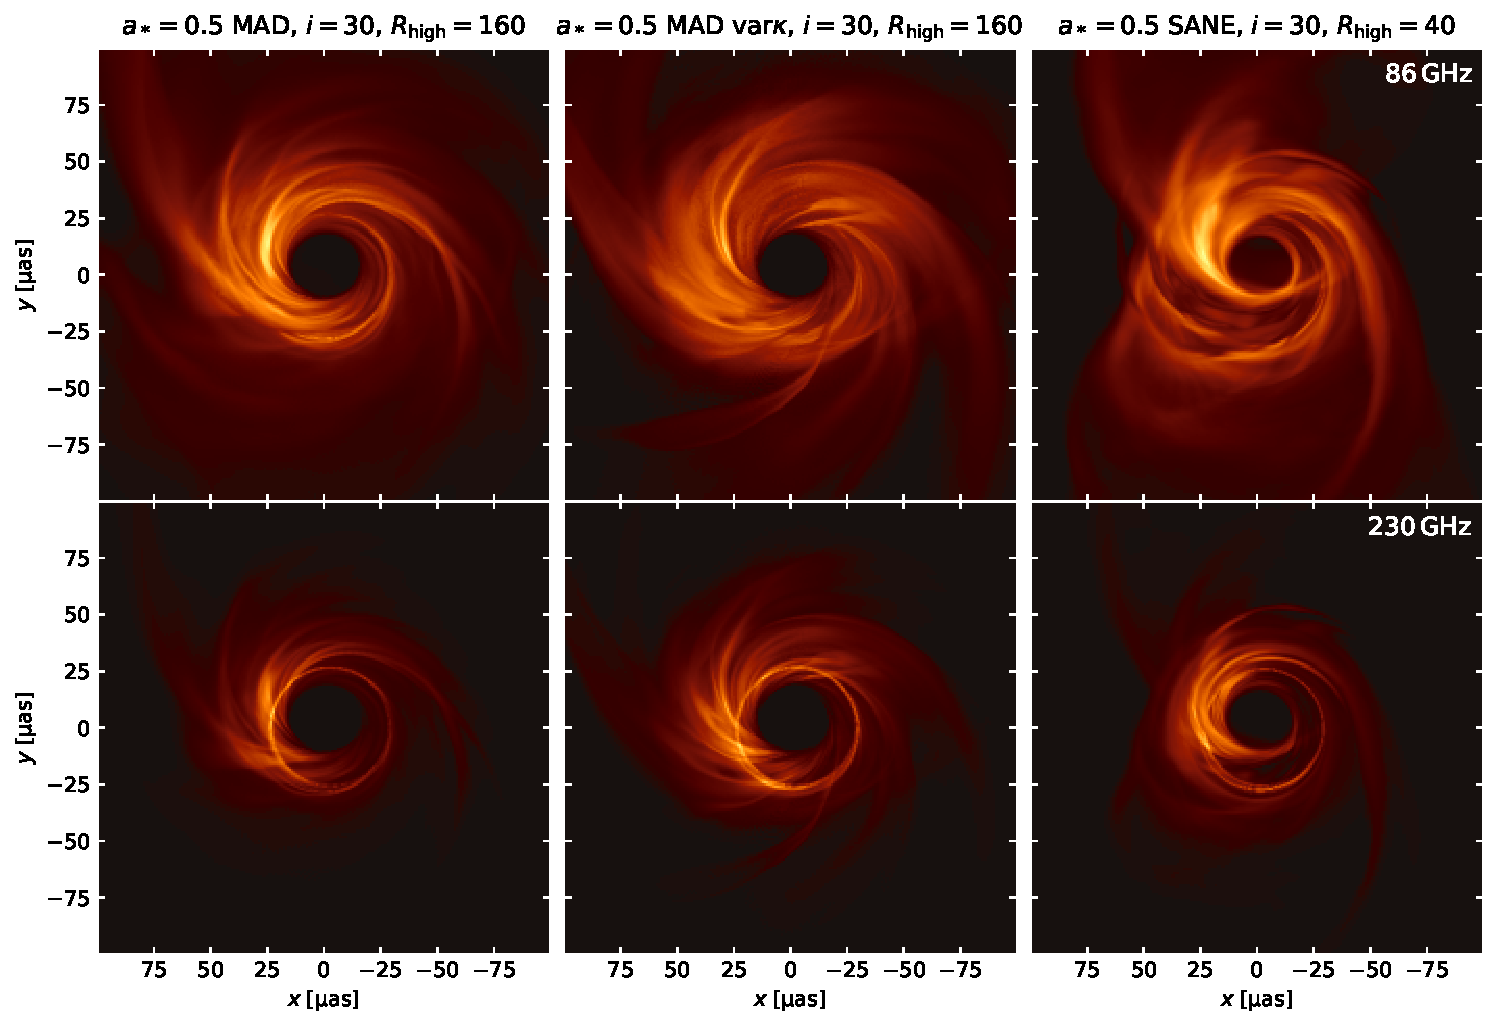
\includegraphics[width=\textwidth]{figures/example_imgs.pdf}
  \caption{Example models from the simulation library.  Left column: best-bet thermal MAD; middle column: nonthermal variable $\kappa$ MAD; right column: thermal SANE model.  Top row: 86\GHz images; bottom row: 230\GHz images.  Color represents intensity, or equivalently brightness temperature.  Angular momentum of the accretion flow projected onto the image points up.  These are relatively successful models satisfying most of the observational  constraints.
  \ckc{will improve 86\GHz resolutions.}}
  \label{fig:example_imgs}
\end{figure*}

\begin{figure*}
  \centering
  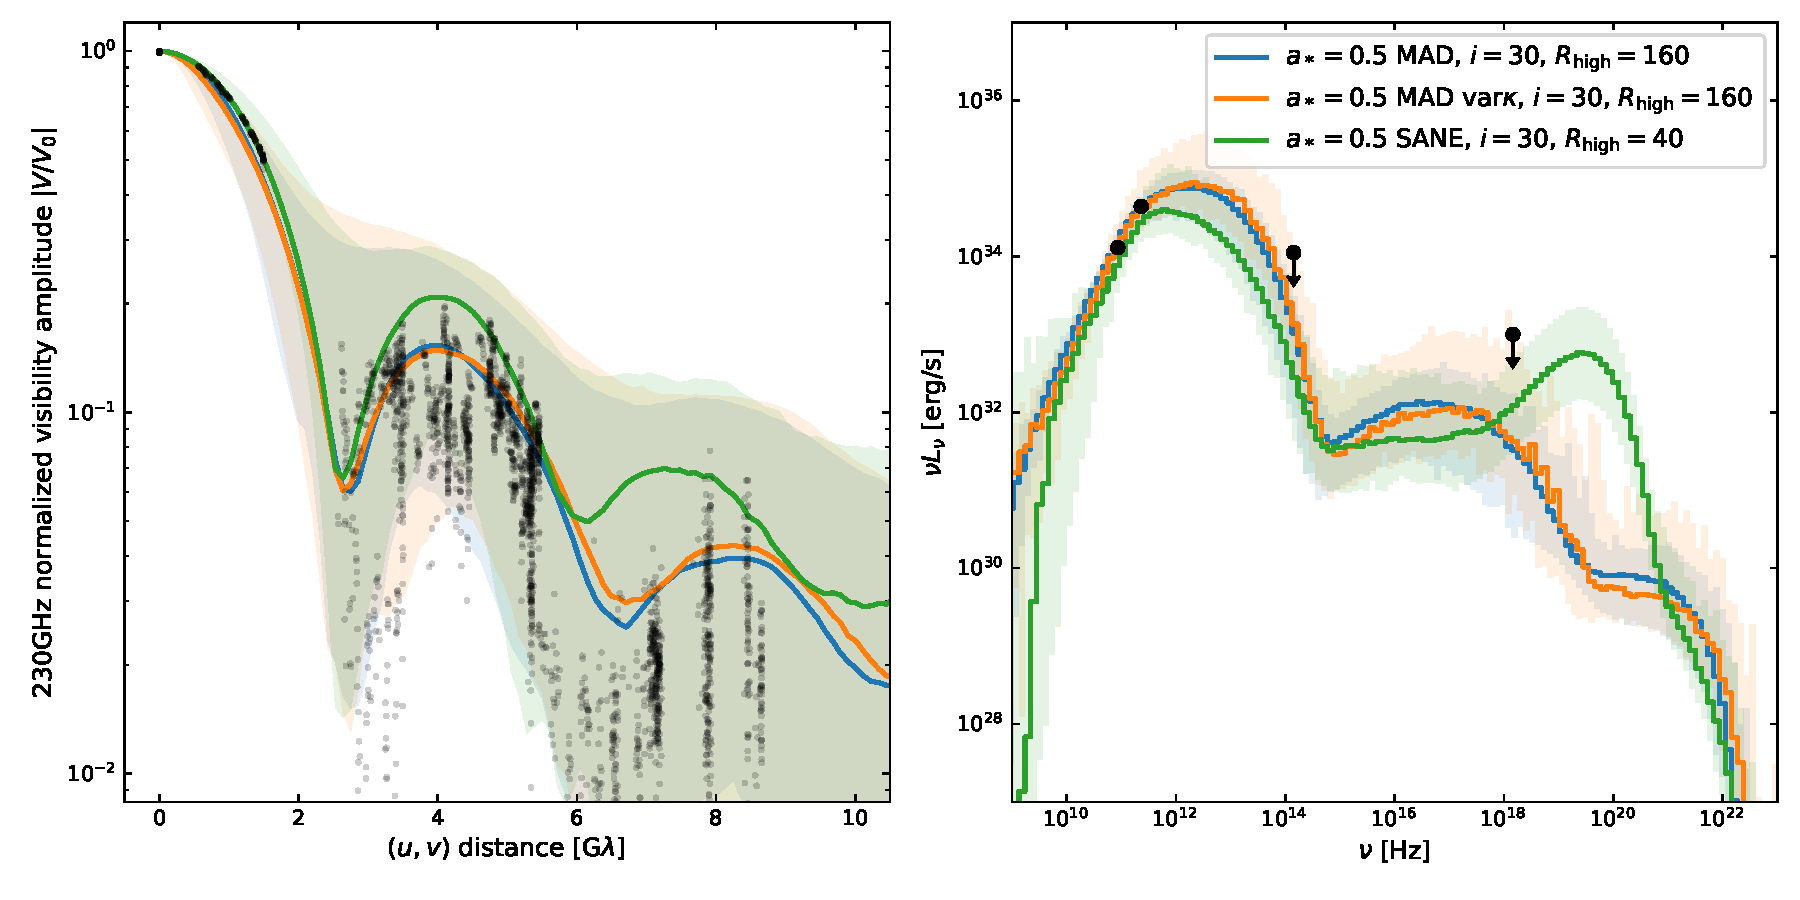
\includegraphics[width=\textwidth]{figures/example_vas_seds.pdf}
  \caption{Visibility amplitudes (left) and SEDs (right) of the three examples, compared with the calibrated EHT~2017 data.  Black symbols show observations.  Blue, orange, and green are the models showed in Figure~\ref{fig:example_imgs} (see also legend for details).  Observed VAs are 1\,minute incoherently averaged data from the HOPS pipeline on \aprilvii.  Model VAs are shown as a solid line for a section at position angle $0\degree$ for a single snapshot, and the band shows the 1st through 99th percentile over all position angles and all times; in this figure no noise is included in the model VAs.  Model SEDs show a solid line for the mean SED and a band for the range across snapshots.}
  \label{fig:example_vas_seds}
\end{figure*}

Given an eDF, density scale $\Munit$, the inclination $i$, and radiative transfer coefficients based on local properties of the plasma, the emergent radiation is obtained by integrating the radiative transfer equation.
We use two classes of numerical methods: ray tracing to generate synthetic images, and Monte Carlo to generate spectral energy distributions (SEDs).

All radiative transport calculations are carried out using the fast light approach, in which plasma variables are read from a single GRMHD dump file and are assumed not to change during ray tracing.
It has been demonstrated by \citet{2010ApJ...717.1092D} (and recently by \citealt{2021MNRAS.508.4282M}) that including light travel effects in the model introduces minor changes to light curves and images.
Further detail on numerical methods is given Appendix~\ref{app:radtrans}.
Comparisons of numerical methods \citep{2020ApJ...897..148G, Prather_et_al_2022} show that differences between radiative transfer schemes do not contribute substantially to the error budget.

The imaged are produced at 86\GHz, 230\GHz and 2.2\um (near infrared, hereafter NIR).
Direct imaging includes synchrotron and bremsstrahlung \citep[both ion-electron and electron-electron; see][for a recent review]{2020ApJ...898...50Y}.  The image library has a typical field of view (full width), resolution (pixel count), and half-width angular size of: $800\uas$, $200 \times 200$, $80 \vartheta_\mathrm{g}$ at 86\GHz; $200\uas$, $400 \times 400$, $20 \vartheta_\mathrm{g}$ at 230\GHz; and $100\uas$, $200\times 200$, $10 \vartheta_\mathrm{g}$ at $2.2\um$.  A few models are imaged with larger field of view or higher resolution.

The SEDs are produced for a set of narrow bins in inclination angle. At each inclination, the SED is averaged over azimuth.  The SED includes synchrotron, bremsstrahlung, \emph{and} Compton scattering.

We find that, although $2.2\um$ emission is usually dominated by synchrotron, occasionally $2.2\um$ synchrotron is so weak that Compton scattering dominates.  We also find that the X-ray can be dominated by either Compton scattering or bremsstrahlung, with the latter dominating in models with a large population of cold electrons at large radius.
Figures~\ref{fig:example_imgs} and \ref{fig:example_vas_seds} show examples of model images and multiwavelength SEDs from our library.

The GRMHD simulation-derived temperatures are unreliable in regions where $\sigma \equiv B^2/(8\pi\rho c^2)$ is large, because truncation error in integration of the total energy equation produces large fractional errors in temperature.  All our radiative transfer models therefore set the emissivity, absorptivity and inverse-Compton scattering cross-sections to $0$ at $\sigma > \sigma_\mathrm{cut} = 1$.

%==============================================================================
\subsection{Summary of \sgra Model Library}

%You can check which data is available here:
%https://docs.google.com/spreadsheets/d/1gw9ichvvYGHLFsZl2wlxqu-O03qEULrwcw3Wixd8BhQ/edit#gid=930351969
%not sure that gives complete answer, but it will help.

A summary of radiative transfer calculations is given in Table~\ref{tab:radiativemodels}. The entire image library contains $6$ simulation sets; thousands of points in model parameter space and $\sim 1.8$M images at each of 86~GHz, 230~GHz, and $2.2\mu$, and $\sim1.3$M SEDs.  The images and SEDs occupy about $50$TB.

We refer to the thermal, $\Rh$ models as ``fiducial'' models, and the remainder as ``exploratory'' models that test the effect of incorporating changes in the eDF or initial conditions.  Nearly all the exploratory models (exceptions are described in the discussion) are imaged over $5 \times 10^3 G M/c^3$, in comparison to $> 10^4 G M/c^3$ for the fiducial models. The sampling noise in the exploratory models is therefore larger than in the fiducial models and they cannot be tested as rigorously as the fiducial models.

For the fiducial models and the variable $\kappa$ models we have multiple, redundant models.  This allows us to control, in part, for uncertainties associated with numerical setup and algorithms.

\begin{deluxetable*}{ccccccc}\label{tab:radiativemodels}
%\tabletypesize{\footnotesize}
\tablecaption{EHT Model Library}
%\renewcommand{\arraystretch}{1.1}
\tablehead{
  \colhead{Simulation}              &%
  \colhead{Transfer Code} &%
  \colhead{$\Rh$}              &%
  \colhead{Inclination}          &%
  \colhead{SED}            &%
  \colhead{$\Delta t/(10^4 GM/c^2)$} &%
  \colhead{Notes}
  }
\startdata
\multicolumn{7}{c}{\bf Fiducial models}\\
\hline
\multicolumn{4}{l}{\it Thermal $\Rh$ models} & &  &\\
\kharma& \ipole & 1, 10, 40, 160 &  10, 30, ..., 170 &  Yes & 15-30 & \\
\bhac  & \bhoss & 1, 10, 40, 160 &   10, 30, ..., 90  &  Yes & 20-30 & \\
\hamr  & \ipole & 1, 40, 160     &   10, 50, 90       &  Yes & 30-35 & \\
\koral & \ipole & 20             &   10, 30, ..., 170 &  No  & 5-100 & \\
\hline
\multicolumn{7}{c}{\bf Exploratory models}\\
\hline
\multicolumn{4}{l}{\it Thermal $\Rh$ models} & &  &\\
\hamr Tilted & \ipole & 1, 40, 160  &  10, 50, 90     &  Yes & 100-103 & \\
Wind Accretion & \ipole & 13, 28  &   N/A     &  No  & 10    &     \\
\hline
\multicolumn{4}{l}{\it Thermal critical $\beta$ model} & & & \\
\kharma & \ipole & 1, 40, 160 &  10, 50, 90 &  No & 30-35 &  \\
\hline
\multicolumn{4}{l}{\it Thermal + power-law models} & & & \\
\hamr &  \ipole & 1, 40, 160 &  10, 50, 90 &  No & 30-35 & $p = 4$ \\
\hline
\multicolumn{4}{l}{\it Thermal + $\kappa$ models} & & & \\
\bhac & \bhoss & 1, 10, 40, 160 &  10, 30, ..., 90 &  No  & 25-30 & $\kappa = 5$ \\
\bhac & \bhoss & 1, 10, 40, 160 &  10, 30, ..., 90 &  No  & 25-30 & $\kappa = 3.5 (\epsilon_0 = 0.05)$\\
\bhac & \bhoss & 1, 10, 40, 160 &  10, 30, ..., 90 &  No  & 25-30 & $ \kappa = 3.5 (\epsilon_0=0.10)$ \\
\bhac & \bhoss & 1, 10, 40, 160 &  10, 30, ..., 90 &  No  & 25-30 & $\kappa = 3.5 (\epsilon_0=0.20)$ \\
\bhac & \bhoss & 1, 10, 40, 80, 160 &  10, 30, ..., 90 &  No  & 25-30 & variable $\kappa=\kappa(\beta, \sigma)$ \\
\hamr & \ipole & 1, 10, 40, 160 &  10, 30, ..., 90 &  Yes & 30-35 & variable $\kappa=\kappa(\beta, \sigma)$ \\
\enddata
\tablecomments{
Summary of the EHT \sgra model library. All models are imaged at $86\GHz$, $230\GHz$, and $2.2\um$ and some (see column 5) also have spectral energy distributions.  For the wind-fed accretion model the viewing angle is set by the stellar orbits and $\Rh$ is set so the model matches the observed 230\GHz flux; $\Rh = 13, 28$ for models with stellar wind magnetizations $\beta = A, B$ respectively \cite{2020ApJ...896L...6R}.
}

\end{deluxetable*}
%\end{rotatetable}
